
%\documentclass[12pt]{article}
\documentclass{article}
%\documentclass[10pt]{article}

%\usepackage{mslapa}
\usepackage{hyperref}
\usepackage{amsmath}
\usepackage{graphicx}
\usepackage{ulem}
%\usepackage{vmargin}
\usepackage{tabularx}
\usepackage{sectsty}
\usepackage{pbox}
\usepackage{bigstrut}
\usepackage{enumerate}
\usepackage{listings}
\usepackage{parskip}   % space paragraphs but dont indent
\usepackage{verbatim}  % \verbatiminput{file}

%\usepackage{cleveref}

%\setpapersize{USletter}
\sectionfont{\normalsize}
\subsectionfont{\normalsize}

% configure \bigstrut size
% This configures spacing above and below rows in a tabularx.
%\renewcommand{\bigstrutjot}{6pt}
\renewcommand{\bigstrutjot}{2.0\jot}

%\setlength{\parindent}{0in}
%\setlength{\parindent}{1.5ex}
%\setlength{\parskip}{1ex plus 0.5ex minus 0.2ex}

\raggedright

\begin{document}

% If a figure is too long to fit in a figure on a single page
% it should got in its own section in the Appendix.

% {{{ Cover Page

\centerline{\bf EECE 311}
\centerline{\bf Fall 2011}
\centerline{\bf}
\centerline{\bf Lab Report \#3}
\centerline{\bf Using SPICE for Th\'{e}venin Circuit Analysis}
%\centerline{\bf Section 4}
%\centerline{\bf 9/13/2011} % date turned in
\centerline{\bf 9/20/2011}  % date lab performed

% signature area
\begin{center}
\begin{tabularx}{\textwidth}[b]{X l l}
Submitted by: & & \\
Signature & Printed Name & Date \\
\hline
\multicolumn{1}{|X|}{} & \multicolumn{1}{|l|}{\bigstrut \bf Jeremiah Mahler} & \multicolumn{1}{|l|}{\bf Oct 4, 2011} \\
\hline
%\multicolumn{1}{|X|}{} & \multicolumn{1}{|l|}{\bigstrut \bf Marvanee Johnson} & \multicolumn{1}{|l|}{\bf Sep 14, 2011} \\
%\hline
\end{tabularx}
\end{center}
% }}}

% Following the instructions for section definitions in the Syllabus
% http://www.ecst.csuchico.edu/~hma/SYL.311.htm

% {{{ Objective
% Puropse of experiment
\section{Objective}

The objective of this lab is to gain experience performing detailed
circuit analysis of a
Th\'{e}venin Equivalant \cite[Pg. 119]{nilsson2008electric} circuit
using SPICE.

% }}}

% {{{ Equipment
\section{Equipment}

To perform the circuit simulation a SPICE\cite{wiki:SPICE} simulator was used.
Specifically, Ngspice\cite{NGSPICE} was used.
But other programs such as Orcad\cite{ORCAD} should also work as well.

%\clearpage
% }}}

% {{{ Procedure
\section{Procedure}

The procedure for this experiment involves two major steps.
\begin{enumerate}
\item Build a SPICE definition of the circuit in Figure \ref{fig:circuit}.
\item Run the simulation and record the output.
\end{enumerate}
For this Th\'{e}venin analysis the open circuit voltage, equivalent
resistance and short circuit current will be found.

\begin{figure}[!hbtp]
\center
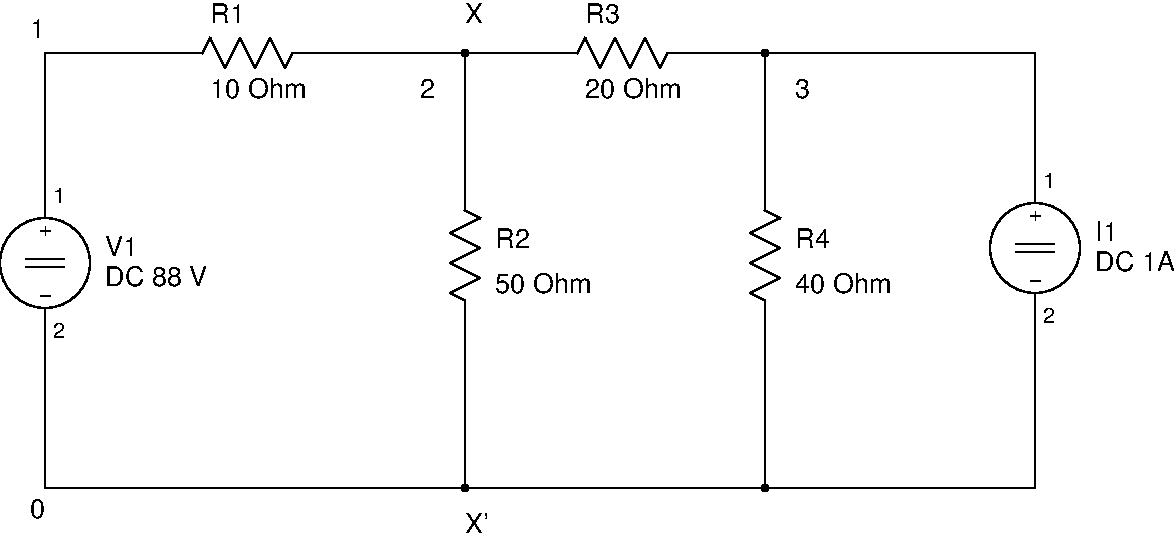
\includegraphics[scale=0.5]{spice/circuit}
\caption{Circuit definition.
Nodes denoted by numbers with 0 as common.
V1 is a voltage source, I1 is a current source.
The Th\'{e}venin Equivalent is calculated with respect to $X$ and $X'$ where
$X$ is positive.
}
\label{fig:circuit}
\end{figure}

\begin{figure}[!hbtp]
\verbatiminput{spice/circuit.cir}
\caption{SPICE definition of circuit in Figure \ref{fig:circuit}.}
\end{figure}

The simulation can be run using Ngspice with the command:
\begin{verbatim}
  ngspice -b your_file.cir
\end{verbatim}
with \verb+your_file.cir+ replaced by the name of your file
containing the SPICE definition.
To save the output to a file a redirect can be used as
in:
\begin{verbatim}
  ngspice -b your_file.cir > your_file.out
\end{verbatim}
If Orcad is being used the same can be accomplished through
its GUI interface.

\clearpage
% }}}

% {{{ Results
\section{Results}

The output of the simulation is shown in Figure \ref{fig:out1}, \ref{fig:out2} and \ref{fig:out3}.
Most of the output is extra information about how long the process took
to run and other things that are of no concern in this lab.
The important values are the open circuit voltage,
short circuit current and Th\'{e}venin resistance.

\begin{figure}[!hbtp]
\verbatiminput{spice/circuit-sc.out}
\caption{Output from SPICE simulation for short circuit current.}
\label{fig:out1}
\end{figure}

\begin{figure}[!hbtp]
\verbatiminput{spice/circuit-tf.out}
\caption{Output from SPICE simulation for Th\'{e}venin equivalent
resistance ("output\_impedance").}
\label{fig:out2}
\end{figure}

\begin{figure}[!hbtp]
\verbatiminput{spice/circuit-voc.out}
\caption{Output from SPICE simulation for open circuit voltage.}
\label{fig:out3}
\end{figure}

\clearpage

% }}}

% {{{ Correlation with theory
\section{Correlation with theory}

To correlate the simulation with theory, manual calculations are
performed here and then they are analyzed at the end of this section.

The first step in this analysis is to simplify the circuit using
source transformation.  The result is show in Figure \ref{fig:circuit-02}.

\begin{figure}[!hbtp]
\center
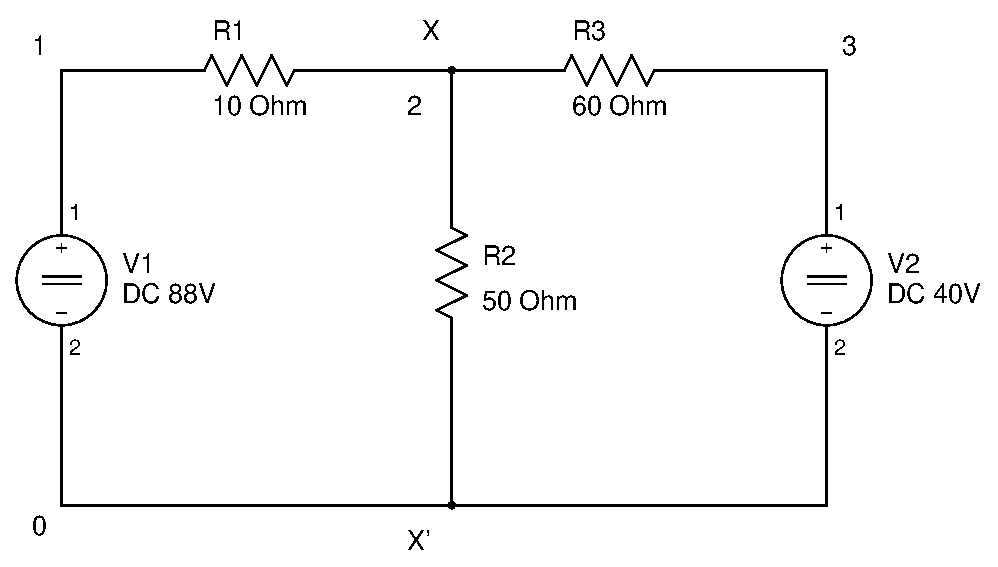
\includegraphics[scale=0.5]{spice/circuit-02}
\caption{Simplification of the circuit (Figure \ref{fig:circuit})
by using source transformation.}
\label{fig:circuit-02}
\end{figure}

Then Node Voltage Analysis can be used to find the open circuit voltage
(Th\'{e}venin Equivalent voltage).
Since $v_1$ and $v_3$ are constant (Figure \ref{fig:circuit-02}) we
only have one equation with one unknown.
\begin{align}
\frac{88 - v_2}{10} + \frac{40 - v_1}{60} + \frac{-v_1}{50} &= 0
\end{align}

Simplifying and substituting results in a Th\'{e}venin voltage of:
\begin{align}
	V_{\mbox{th}} &= v_2 \\
	              &= 69.268 \quad \mbox{[volts]}
\end{align}

The Th\'{e}venin equivalent resistance can be found by finding the resistance
when both voltage sources are disabled (0 volts).
This is equivalent to all the resistors in parallel.

\begin{align}
	R_{\mbox{th}} &= \frac{1}{ 1/10 + 1/50 + 1/60} \\
				  &= 7.317 \quad \mbox{[ohms]}
\end{align}

The Th\'{e}venin equivalent voltage and resistance found in these
calculations were 69.268 volts and 7.317 ohms respectively.
The Th\'{e}venin equivalent voltage and resistance found from
the SPICE simulation were 69.268 volts (Figure \ref{fig:out3})
and 7.317 ohms (Figure \ref{fig:out2}) respectively.
These values are identical indicating that the theory corresponds
exactly with the simulation.

%\clearpage
% }}}

% {{{ Conclusion
\section{Conclusion}

This experiment was a complete success in performing a detailed
circuit analysis of a Th\'{e}venin Equivalent circuit
using SPICE.
The calculations matched the theoretical values exactly
with no measurable amount of error.

% }}}

% {{{ References
\clearpage

\pagebreak
\renewcommand*{\refname}{\vspace{-8mm}}
\section{References}
\bibliographystyle{ieeetr}
\bibliography{../references}
% }}}

\end{document}

% vim:foldmethod=marker

